\documentclass[11pt, oneside]{article}
\usepackage{geometry}
\geometry{letterpaper}
\usepackage{graphicx}
\usepackage{enumitem}
\usepackage{fullwidth}		
\usepackage{amssymb}
\usepackage{fancyvrb}
\usepackage{color}
\usepackage{floatrow}
\usepackage{hyperref}
\setlength\parindent{0pt}
\hypersetup{
    colorlinks,
    citecolor=green,
    filecolor=black,
    linkcolor=blue,
    urlcolor=blue
}
\title{Assignment 2}
\author{Pipob Puthipiroj}
\begin{document}
\date{}
\maketitle

\section*{Question 1}
Write your own original code that produces a dataset that conforms to the classic univariate regression model. Your data set should have 99 observations and a Normal error term. The slope of the coefficient on your regressor should be positive. Now include a single outlier, such that when you fit a regression to your 100 data points, the slope of your regression line is negative.  Your answer to this question should consist of:
\begin{enumerate}[label=(\alph*)]
	\item Your original data-generating equation 
	\item Regression results for the original 99 (copy/paste the ``summary" output) 
	\item Regression results with the outlier included (copy/paste ``summary" output)
	\item A properly-labeled data visualization that shows a single scatterplot, the regression line based on the original 99 points, and another differentiated regression line based on 100 points.
	\item No more than 3 sentences that would serve as a caption for your figure if it were to be included in an econometrics textbook to illustrate the dangers of extrapolation.
	\end{enumerate}
	\section*{Full Code}
	All code for the assignment can be found \href{https://github.com/thetruejacob/CS112/blob/master/Assignment/Assignment\%202.ipynb}{here}.
	\begin{verbatim}
set.seed(1)
x = c(rnorm(n = 99, mean = 0, sd = 1), 3)
y = c(0.5*x[-100] + rnorm(n = 99, mean = 0, sd = 1), -30)
summary(lm(y[1:99] ~ x[1:99]))
summary(lm(y ~ x))

plot(y ~ x)
abline(lm(y[-100] ~ x[-100]), col = "red")
abline(lm(y ~ x), col = "blue")
\end{verbatim}
\newpage
\section*{Regression Results}
\begin{verbatim}
Call:
lm(formula = y[1:99] ~ x[1:99])

Residuals:
    Min      1Q  Median      3Q     Max 
-1.8988 -0.5718 -0.1101  0.5678  2.2892 

Coefficients:
            Estimate Std. Error t value Pr(>|t|)    
(Intercept) -0.03465    0.09774  -0.355 0.723702    
x[1:99]      0.42479    0.10816   3.927 0.000161 ***
---
Signif. codes:  0 '***' 0.001 '**' 0.01 '*' 0.05 '.' 0.1 ' ' 1

Residual standard error: 0.9646 on 97 degrees of freedom
Multiple R-squared:  0.1372,	Adjusted R-squared:  0.1283 
F-statistic: 15.42 on 1 and 97 DF,  p-value: 0.0001609 
\end{verbatim}  

\mbox{}\\

\begin{verbatim}
Call:
lm(formula = y ~ x)

Residuals:
     Min       1Q   Median       3Q      Max 
-28.0233  -0.6306   0.1935   0.9965   4.6926 

Coefficients:
            Estimate Std. Error t value Pr(>|t|)  
(Intercept)  -0.2010     0.3176  -0.633   0.5282  
x            -0.5919     0.3351  -1.766   0.0804 .
---
Signif. codes:  0 '***' 0.001 '**' 0.01 '*' 0.05 '.' 0.1 ' ' 1

Residual standard error: 3.139 on 98 degrees of freedom
Multiple R-squared:  0.03086,	Adjusted R-squared:  0.02097 
F-statistic:  3.12 on 1 and 98 DF,  p-value: 0.08043
\end{verbatim} 
\newpage
\section*{Data Visualization and Caption}
\begin{figure*}[h]
	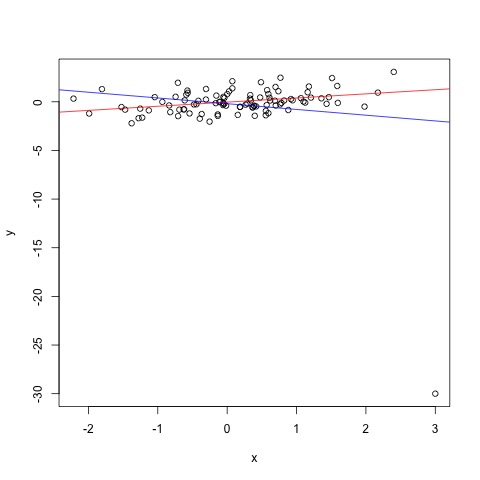
\includegraphics[width = 8cm, height = 8cm]{q1.jpg}
\end{figure*}
We see that when excluding the outlier in the bottom right, the regression line (in red) is slightly positive, with a highly significant $p$-value of 0.000161 and an $R^2$ of 0.1372, meaning 13\% of the variability in y is explanable by x using this line. When the outlier is included, the best fit line re-optimizes and becomes negative. However, the fit using this line is far poorer, as the $p$-value is now a non-significant $p = 0.08 \geq 0.05$, and the $R^2$ is now 0.03, making the 'best-fit line' barely better than a horizontal line.\footnote{\#regression: I use the regression equation to provide an interpretation of the relationship between x and y, and explain how the introduction of the outlier produces a far worse regression that is not easily recognized in the plot.}

\newpage
\section*{Question 2} NOTE: FOR THIS PROBLEM (AND THIS PROBLEM ONLY), USE ONLY THE CONTROL GROUP. DO NOT USE ANY UNITS FOR WHICH TREATMENT == 1.
Using the Lalonde data set and a linear model that predicts re78 as a linear additive function of age, educ, re74, re75, educ*re74, educ*re75, age*re74, age*re75, and re74*re75, estimate:
\begin{enumerate}
	\item the 95\% prediction interval for re78, for every unit (i.e., each age, spanning the age range in the data set), using simulation (i.e., 10000 simulated predictions for every row from 10000 sets of coefficients). You will need to incorporate simulated sigmas, and you should hold educ, re74, and re75 at their medians (hence only age will vary). 
	\item the 95\% prediction interval for re78, for every unit, using simulation (i.e., 10000 simulated predictions for every row from 10000 sets of coefficients). You will need to incorporate simulated sigmas, and you should hold educ, re74, and re75 at their 90\% quantiles (hence only age will vary).
\end{enumerate}
Your answer to this question should consist of the following:


\begin{enumerate}[label=(\alph*)]
	\item A table with the relevant point estimates (e.g., the bounds of the prediction intervals of y for the different ages, and the medians of the other predictors)
	\item 2 figures showing the scatterplots (one for the analysis holding predictors at their medians, and other for the analysis holding predictors at their 90\% quantiles). The ``scatterplots" don't have to show the original data--all I am interested in are the prediction intervals for each age. Each of these figures should show how the prediction intervals' change over time (i.e., over the range of ages in the data set). Be sure to label your plot's features (axis, title, etc.). \\ \\ E.g.: https://gist.github.com/diamonaj/75fef6eb48639c2c36f73c58d54bac2f
\end{enumerate}
\section*{Tables}
The full tables are accessible \href{https://github.com/thetruejacob/CS112/blob/master/Assignment/Assignment\%202.ipynb}{here}.
\begin{table}[h]
\begin{tabular}{|l|l|}
\hline
\textbf{2.5\%} & \textbf{97.5\%} \\ \hline
-6910.046      & 15014.98        \\ \hline
-6905.489      & 15019.01        \\ \hline
-6916.160      & 14999.72        \\ \hline
-6872.834      & 15040.22        \\ \hline
-6874.963      & 15070.68        \\ \hline
-6891.289      & 15005.63        \\ \hline
\end{tabular}
\end{table}
\section*{Prediction Intervals}
\begin{figure*}[h]
	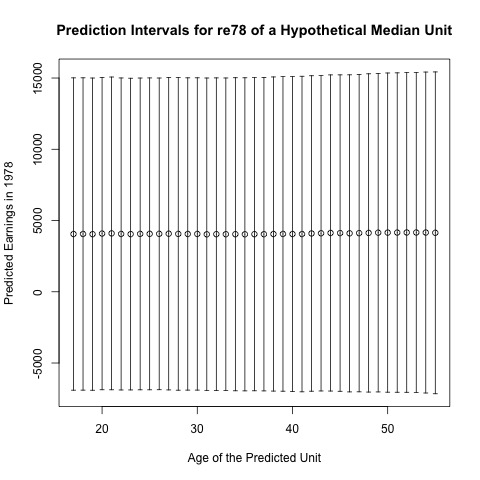
\includegraphics[width = 7cm, height = 7cm]{medianplot.jpg}
	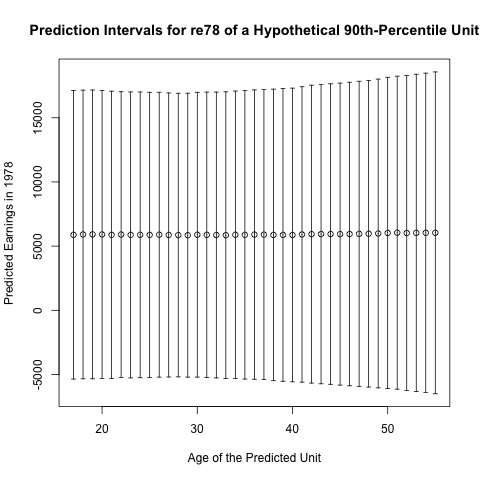
\includegraphics[width = 7cm, height = 7cm]{ninetyplot.jpg}
\end{figure*}
Unsurprisingly, the hypothetical 90th percentile individual (who has 90th percentile levels of education and real earnings in 1974 and 1975) is predicted to earn more in 1978 (a mean of over \$5000) than a hypothetical $50^\textrm{th}$ percentile, or median individual, whose mean prediction is below \$5000. Interestingly, the older the predicted individual, the greater the variability in predicted 1978 earnings for the $90^\textrm{th}$ percentile unit, although the mean of the prediction interval stays relatively constant. The same pattern can be seen in the median unit, although it is much more subdued.\footnote{\#decisiondesign: In the control group, there are no samples which have certain ages for which we can directly make predictions. Therefore, we instead 10,000 bootstrapped samples for every age, and use the 2.5 and 97.5 percentiles of those predictions  for each of the 39 ages to understand the precision of our estimate.}\footnote{\#dataviz: I generate a detailed data visualization for re78 prediction intervals for both the hypothetical median unit, as well as the 90th percentile unit, and give a detailed insight into what the differences are.}
\newpage
\section*{Question 3}
Obtain the \textit{nsw.dta} dataset from http://users.nber.org/~rdehejia/data/nswdata2.html. Read the description of this data set provided on the page. If you proceed with this work in R (recommended) use the \textit{foreign} library to open it (so you can use \textit{read.dta}). \\ 

Specify a regression model in which the dependent variable is re78 and the sole predictor is treatment (and, an intercept should be included automatically, by default). Then, bootstrap the 95\% confidence intervals for the value of the coefficient for treatment. Then, obtain the analytical confidence interval for the coefficient value using the standard error that pops out of a regression (or equivalently, in R, you can use the \textit{confint} function). Compare the two confidence intervals--one obtained via simulation, the other via the formula.\\

\textbf{NOTE: Make sure that you don't use a `canned' bootstrap function -- please code the bootstrap routine manually.}\\

Your answer to this question should consist of the following:
\begin{itemize}
\item A table with the relevant results (bounds on the 2 confidence intervals).
\item 1 histogram (properly labeled) showing your bootstrap-sample results. How you do this one is up to you.
\item No more than 3 sentences summarizing the results and drawing any conclusions you find relevant and interesting.
\end{itemize}

\section*{Confidence Intervals}
The full code for this question is accessible  \href{https://github.com/thetruejacob/CS112/blob/master/Assignment/Assignment 2.ipynb}{here}.
\begin{table}[h]
\begin{tabular}{l|l|l|}
\cline{2-3}
                                          & \textbf{2.5\%} & \textbf{97.5\%} \\ \hline
\multicolumn{1}{|l|}{\textbf{bootstrap}}  & -57.17378      & 1861.711        \\ \hline
\multicolumn{1}{|l|}{\textbf{analytical}} & -40.52635      & 1813.134        \\ \hline
\end{tabular}
\end{table}
\newpage
\section*{Histogram}
\begin{figure*}[h]
	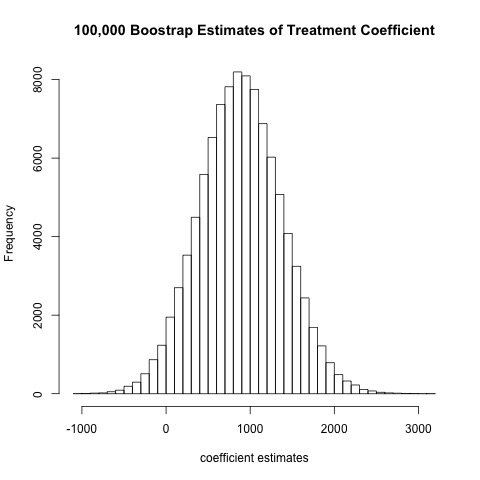
\includegraphics[width = 7cm, height = 7cm]{coefestimates.jpg}
\end{figure*}
With enough bootstrap estimates, we see that the estimates of the treatment coefficients are normally distributed around 880. In other words, if we did not know anything about the participants besides their treatment status, our estimate for the impact of the treatment is only around \$900. Based only on this limited information, we cannot say if the true effect (ATT) is higher or lower than this figure, because we can determine neither the magnitude nor even the sign of the selection bias.\footnote{\#decisiontheory: I explain how the figure alone is not helpful in determining the true effect of the Lalonde program, as this figure does not take selection bias into account and outputs $E[Y^T_i|T] - E[Y^C_i|C]$.}

\section*{Question 4}
Write a function (5 lines max) that takes Ys and predicted Ys as inputs, and outputs $R^2$. Copy/paste an example using the \textit{nsw.dta} data (from \#3 above) that shows it working.
\begin{verbatim}
r2 = function(y, f){
    rss = sum((y - f)^2)
    tss = sum((y - mean(y))^2)
    1 - rss/tss
}
r2(df$re78, predict(lm(re78 ~ treat, data = df)))	 #0.00487157134050964
summary(lm(re78 ~ treat, data = df))$r.squared		    #0.00487157134050952
\end{verbatim}\footnote{\#algorithms: Clear, concise code for calculating $R^2$ as $1 - SS_{res}/SS_{tot}$.}

\newpage
\section*{Question 5}
Use the nsw.dta dataset from question 3 above to estimate the probability of being assigned to the treatment group (vs. the control group) for every observation in the data set. Your logistic regression model should be a linear additive function of all predictors available to you -- no interaction terms needed. NOTE: re78 is not a predictor because it postdates the treatment. (In other words, it's an outcome.) \\ \\ 
Your answer to this question should consist of the following:
\begin{enumerate}[label=(\alph*)]
\item Two properly labeled histograms: one in red (showing the distribution of the treatment group's estimated probabilities) and one in blue (showing the distribution of the control group's estimated probabilities). Extra credit for a legend in the plot.
\item No more than 3 sentences summarizing the differences between the two distributions of estimated probabilities, and whether/not your results are surprising and/or intuitive.
\end{enumerate}
\begin{figure*}[h]
	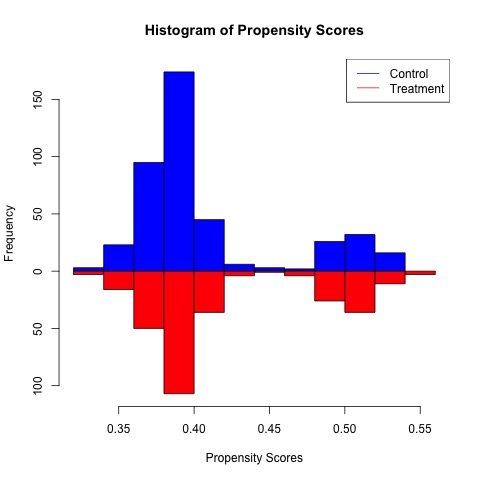
\includegraphics[width = 8cm, height = 8cm]{propensity.jpg}
\end{figure*}
Surprisingly, the propensity scores of both the treatment and control populations are bimodal, with a peak at 0.38 and at 0.52, with very little mass at the midpoint at 0.45. There is slightly more mass in the upper peak for the treatment group, and more in the lower peak for the control, which is intuitive. However, that the propensity scores of the entire population are between the narrow range of 0.33 and 0.55 is quite surprising.\footnote{\#dataviz: I believe this to be quite a clear way of comparing the positivity of the dataset.}


\newpage
\section*{Optional: Question 6}
Write code that repeatedly randomly selects predictors from the lalonde data set, runs a regression on those predictors (with ``re78"	 as the dependent variable), and saves the treatment effect.  Produce a histogram showing the wide range of treatment effects that pop out. (This is much easier if you exclude interaction effects). Produce another histogram that shows the wide range of treatment effects that pop out that are also statistically significant.
\begin{figure*}[h]
	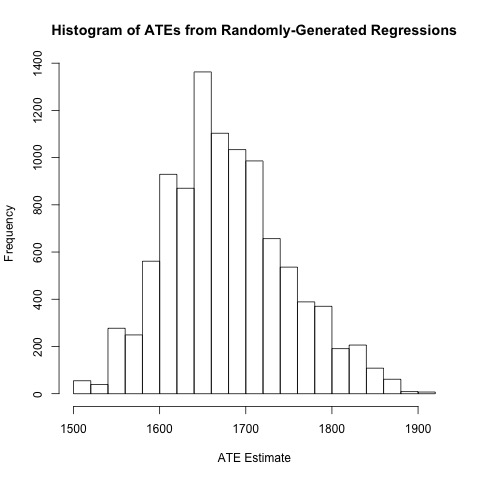
\includegraphics[width = 7cm, height = 7cm]{atehist.jpg}
	
\includegraphics[width = 7cm, height = 7cm]{histatt.png}
\end{figure*}
Even when the regression is run 10,000 times, the treatment effects do not follow a nice distribution. It is quite approximately a normal distribution with a mean at 1660. There was no difference between the histogram of treatment effects, and significant treatment effects, as all effects were significant. The distribution of the right is obtained by randomly choosing a random number of predictors, running a matching algorithm and estimating ATT.W hen performing propensity score matching and randomizing predictors, a much smoother, and likely more accurate estimate is obtained, with an approximately normal distribution centered around 1711, showing considerable agreement between both graphs that the Lalonde Program.
\footnote{\#decisionanalysis: After recognizing the flaws of using a randomly generated simple regression to estimate the ATT, I implemented a more rigorous to perform matching before estimating ATT for each set of randomly-generated predictors.}
\footnote{\#algorithms: The code used for obtaining the graph on the right was not at all easy, as it required a for-loop over a matching function (via MatchIt) and ATT estimation (via Zelig). The whole code for 100,000 loops took around 3 hours to run.}
\footnote{\#observationalstudy: I offer two methods in order to interpret Lalonde's findings: first by running a regression with randomly generated predictors, with does not account for selection bias, and the other by running a matching algorithm with random predictors, which does. This allows me to much more rigorously pin the true treatment effect size down to about 1711, with a standard deviation of 200.}



\end{document}

